%% LyX 2.2.2 created this file.  For more info, see http://www.lyx.org/.
%% Do not edit unless you really know what you are doing.
\documentclass[english]{article}
\usepackage[T1]{fontenc}
\usepackage[latin9]{inputenc}
\usepackage{float}
\usepackage{graphicx}

\makeatletter

%%%%%%%%%%%%%%%%%%%%%%%%%%%%%% LyX specific LaTeX commands.
%% Because html converters don't know tabularnewline
\providecommand{\tabularnewline}{\\}

\makeatother

\usepackage{babel}
\begin{document}

\part{ELECTRO III EJERCICIO 2}

\section{Compatibilidad entre Compuertas}

Al momento de adquirir una compuerta l�gica comercial, se especifica
en el c�digo el tipo de tecnolog�a que se implementa en dicha compuerta.
Por ejemplo, ``HC'' hace referencia a ``High speed CMOS'' mientras
que ``HCT'' significa ``High speed CMOS TTL'' o tambi�n existe
``LS'' aludiendo a ``Low power schotky''. En esta parte del art�culo
se analizaran algunas diferencias pr�cticas entre estos tipos compuertas
y se mencionaran algunos par�metros a tener en cuenta para combinar
m�s de dos tipos disitintos en un mismo circuito.

Para el an�lisis se utilizar�n las siguientes compuertas l�gicas:
74HC02, 74HCT02, 74LS02. Estas corresponden a compuertas ``NOR''.

\subsection{Margen de Ruido}

De la hoja de datos de los distintos componentes se extrajeron los
siguientes par�metros sobre el margen de ruido:

\begin{table}
\begin{tabular}{|c|c|c|c|}
\hline 
 & 74HC02 & 74HCT02 & 74LS02\tabularnewline
\hline 
High Level Noise Margin &  &  & \tabularnewline
\hline 
Low Level Noise Margin &  &  & \tabularnewline
\hline 
\end{tabular}

\caption{Margenes de Ruido - Extra�dos de Hojas de Datos}

\end{table}


\subsection{Conexi�n entre Compuertas}

Al conexionar entre compuertas, pueden existir problemas al cargar
la tecnolog�a LS con una compuerta de tipo HC. Esto es debido a que
los niveles de entrada (como se puede observar en la tabla expuesta
anteriormente) de la tecnolog�a HC son m�s restrictivos que los valores
de salida de la LS. Por otro lado, este problema no ocurre cuando
se carga la compuerta LS con una HCT, la cual justamente est� pensada
para solucionar los problemas de compatibilidad de una HC.

De todas maneras, aunque el fabricante en la datasheet de su componente
indique valores como los que se han mostrado en el apartado anterior,
en la pr�ctica puede ocurrir que estos par�metros difieran como por
ejemplo en el caso del margen de ruido. Es decir, que puede ocurrir
que en la pr�ctica se pueda interconectar una compuerta LS con una
HC sin tener problemas debido a que el margen de ruido de la LS sea
m�s elevado de lo que se indica en la hoja de datos. A continuaci�n
se muestra una imagen de una medici�n realizada con osciloscopio de
la respuesta de una compuerta LS cargada por una HC:

\begin{figure}[H]
\begin{centering}
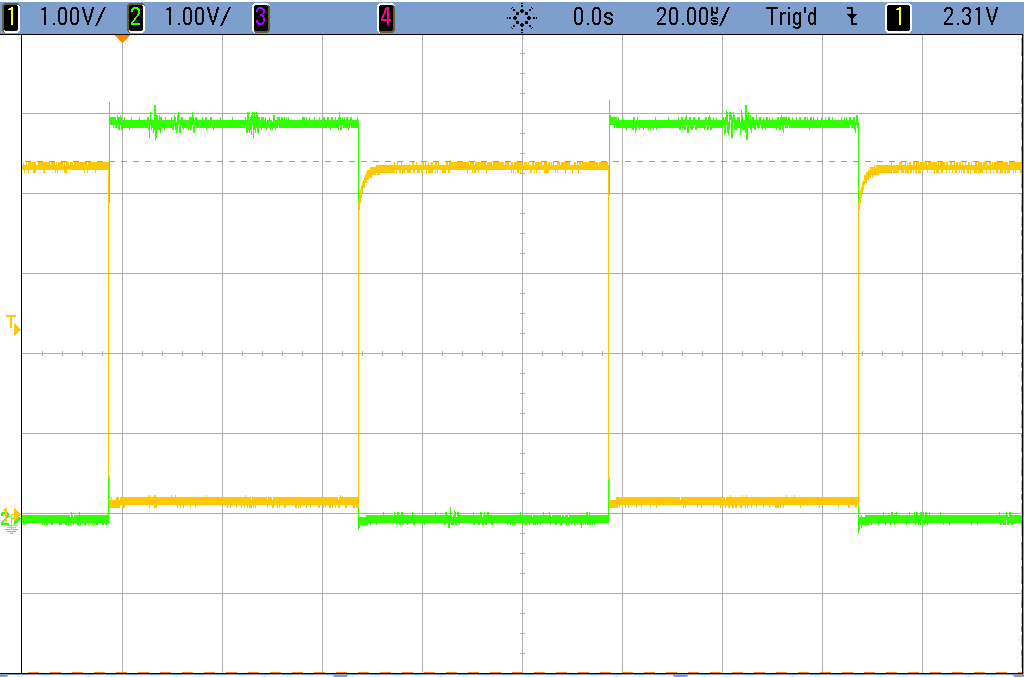
\includegraphics[scale=0.4]{LS-CargadoConHC02}
\par\end{centering}
\caption{Medici�n - Compuerta LS cargada con HC}
\end{figure}

Las compuertas son NOR que se conexionaron de tal manera que simulan
dos NOT en serie, por ende tiene sentido que cuando una se�al est�
en alto la otra se mantiene en bajo. Vale aclarar que la se�al representada
de color amarillo es la salida de la compuerta HC mientras que la
otra es la correspondiente a la compuerta LS.
\end{document}
